% MidtermExam.tex
% by Erin Kiley <emkiley at mcla dot edu>
% July 03, 2017
% This file is licensed under a Creative Commons Attribution-ShareAlike 3.0 United States License ( https://creativecommons.org/licenses/by-sa/3.0/us/ )
% 
% This file serves as a template for midterm exams (the difference between midterm and final exams is the placement of the points table; since finals won't be handed back, scores can be written on the front page). It automatically computes the number of problems and number of possible points, and automatically typesets the points table.
%
% Run latex on this file at least twice in order to get the page numbers and point counts correct.

\documentclass[letterpaper,12pt]{article}

\usepackage{enumitem} % for customized \item command in lists
\usepackage{verbatim} % for the \begin{comment}...\end{comment} environment
\usepackage{amssymb,amsmath} % for math symbols

% Margins
\usepackage{simplemargins} % available from https://www.scath.net/ws_2011/abstract-templates/simplemargins.sty/at_download/simplemargins.sty
\setallmargins{0.75in}
\setbottommargin{1in}

% Mathy commands
\providecommand{\abs}[1]{\left\vert{#1}\right\vert}
\providecommand{\dabs}[1]{\abs{\abs{#1}}}
\providecommand{\inv}[1]{{#1}^{-1}}
\providecommand{\st}{\ensuremath{\;:\;}}
\providecommand{\D}{\ensuremath{\;\mathrm{d}}}
\providecommand{\eps}{\ensuremath{\varepsilon}}
%\providecommand{\R}{\ensuremath{{\mathbb{R}}}}
\providecommand{\R}[1][]{\ensuremath{\R^{#1}}} % \R[2] produces $\mathbb{R}^2$, whereas \R produces just $\mathbb{R}$
\providecommand{\Rn}{\ensuremath{{\R^n}}}
\providecommand{\Z}{\ensuremath{{\mathbb{Z}}}}
\providecommand{\N}{\ensuremath{{\mathbb{N}}}}
\providecommand{\code}[1]{\fvset{frame=single,numbers=left, numbersep=3pt}\VerbatimInput{#1}}

% For making plots
\usepackage{mathtools}
\usepackage{tikz}
\usepackage{pgfplots}% Uses tikz
\pgfplotsset{compat=newest}% use newest version
\usepgflibrary{fpu}
\usetikzlibrary{calc}
\tikzset{My Line Style/.style={smooth, thick, samples=400}}
\usepackage{xcolor} %Additional colors
\pgfplotsset{every axis/.append style={
                    axis x line=middle,    % put the x axis in the middle
                    axis y line=middle,    % put the y axis in the middle
                    axis line style={<->,color=blue}, % arrows on the axis
                    xlabel={$x$},          % default put x on x-axis
                    ylabel={$y$},          % default put y on y-axis
            }}

% For plotting little normal curve
\pgfmathdeclarefunction{gauss}{2}{\pgfmathparse{1/(#2*sqrt(2*pi))*exp(-((x-#1)^2)/(2*#2^2))}}

\newcommand{\normalcurve}{
	\begin{tikzpicture}
	\begin{axis}[no markers, domain=0:10, samples=100,
	axis lines*=none,
	xlabel=$x$, ylabel=$y$,
	height=4cm, width=8cm]
	\addplot [domain=-3:3] {gauss(0,1)} \closedcycle;
	\end{axis}
	\end{tikzpicture}
	}

% For typesetting solutions
\providecommand{\sol}[1]{\vskip0.5em
\fbox{\begin{minipage}{0.9\textwidth}
\noindent{\textbf{Solution.~}}
#1
\end{minipage}}\vskip0.5em
}

\providecommand{\continuesol}[1]{\vskip0.5em
\fbox{\begin{minipage}{0.9\textwidth}
\noindent{}
#1
\end{minipage}}\vskip0.5em
}

% Space for a short answer
\providecommand{\shortans}{\vskip9em}

% Space for a long answer
\providecommand{\longans}{\vskip15em}

% Set up counters for page numbers, problems, points
\usepackage{totcount}

\def\computemycount{}
\expandafter\ifx\csname Counters\endcsname\relax
\usetotcountfile{Counters.aux}
\newcounter{mycount} % so that increments of this counter don’t break
\else
\newtotcounter[auxfile=Counters.aux]{PointCount}
\newtotcounter[auxfile=Counters.aux]{ProbCount}
\newtotcounter[auxfile=Counters.aux]{BonusCount}\fi

\newtotcounter{PointCount}
\newtotcounter{ProbCount}
\newtotcounter{BonusCount}
\regtotcounter{page}

\usepackage{calc}
\newcounter{TotalProbs}
\newcounter{TotalSheets}


% Command for a problem
\providecommand{\prob}[1]{ %
\stepcounter{ProbCount} %
\addtocounter{PointCount}{#1} %
\item \textbf{[{#1} points]} %
\immediate\write\pointstable{\arabic{enumi} (#1 pts) \unexpanded{&\quad\quad\quad\quad\quad\quad\\ &\\ \hline}}
}

% Command for a bonus problem
\providecommand{\bonusprob}[1]{ %
\stepcounter{BonusCount} %
\item \textbf{[{#1} bonus points]} %
\immediate\write\pointstable{\arabic{enumi} (#1 BONUS pts) \unexpanded{&\quad\quad\quad\quad\quad\quad\\ &\\ \hline}}
}


\begin{document}

% FRONT PAGE
\noindent MATH 232 \hfill Name: \rule{20em}{0.5pt}\\
\noindent Instructor: E.M.\ Kiley\\
\noindent May 5, 2017 \hfill  Section \textbf{(circle one)}: $\quad$ 01 (10 a.m.) $\qquad$ 02 (1 p.m.)\\
\begin{center}\textbf{Exam 3}\end{center}
\topskip0pt
\vspace*{\fill}

% Compute total number of problems (regular + bonus)
\setcounter{TotalProbs}{\totvalue{ProbCount}+\totvalue{BonusCount}}

% Compute total number of sheets (assumes two-sided printing)
\ifodd\totvalue{page}
	\setcounter{TotalSheets}{\totvalue{page}/2+1}
\else
	\setcounter{TotalSheets}{\totvalue{page}/2}
\fi

% Print rules and guidelines for exam
\begin{center}
\fbox{
\begin{minipage}{0.8\textwidth}
\vskip0.1em
\begin{center}{\Large{\textbf{ATTENTION:}}}\end{center}
\begin{enumerate}[label=\textbf{\Roman*)}]
\item This exam consists of \total{page} pages and is printed front-and-back on \arabic{TotalSheets} sheets of paper, with \arabic{TotalProbs} total problems, including \total{ProbCount} required problems and \total{BonusCount} bonus. Make sure you have the correct number of pages and problems.
\item No books, notes, calculators, or other tools may be used on the exam.%, except for your one 8.5''$\times$11'' cheat sheet. \textbf{You must submit your cheat sheet along with your exam.}
\item {\Large\textbf{Show all work clearly and in logical order}.} Explain your answers using full English sentences. A correct answer without appropriate work will receive little or no credit.
\item Simplify your answers as much as you can without a calculator, and show all your work.
\item You will find scrap paper in the front of the classroom, and you are to use \emph{only} this paper for your scratch work; do not use any of your own paper.
\item If you have scrap paper that you would like to submit along with your exam, then please use the stapler at the front of the classroom to attach it to your work.
\item The exam time will be two hours. \textbf{Good luck!}
\end{enumerate}
\end{minipage}
}
\end{center}
\vspace*{\fill}

\pagebreak

% Print the points table
\topskip0pt
\vspace*{\fill}
\IfFileExists{./\jobname-pointstable}{\input{\jobname-pointstable}}{typeset again to get points table}
\vspace*{\fill}

\pagebreak


\begin{enumerate}[label=\textbf{Problem \arabic*.},resume]
% Begin writing points table in separate tex file-------------
\newwrite\pointstable
\immediate\openout\pointstable=\jobname-pointstable.tex
\immediate\write\pointstable{\unexpanded{\begin{center}\begin{tabular}{|l|l|}\hline\textbf{Problem} & \textbf{Score}\\&\\ \hline }}
%--------------------------------------------------------------

% EXAM CONTENT

\prob{8} Lorem ipsum
	\begin{enumerate}[label=\textbf{(\alph*)}]
	\item Consider the astroid shown in the figure below, and defined by the equations
	\begin{equation*}
	x=\cos^3t,\qquad y=\sin^3t,\qquad0\leq t\leq2\pi.
	\end{equation*}
	
		\centerline{
        \begin{tikzpicture}
            \begin{axis}[
                    xmin=-1.1,xmax=1.1,
                    ymin=-1.1,ymax=1.1,
                    grid=none,
                    ]
                    \addplot [domain=0:2*pi,samples=50]({(cos(deg(x)))^3},{(sin(deg(x)))^3});
            \end{axis}
        \end{tikzpicture}
        }
	\item Subsequent parts of a multipart problem\vfill
	\end{enumerate}

\prob{24} A whole bunch of cute little normal curves
	\begin{enumerate}[label=\textbf{(\alph*)}]
	\item $P(X>1.5)$ or $P(X>2)$
	
	\normalcurve
	
	\item $P(X<-1.5)$ or $P(X<-2)$

	\normalcurve
	
	\item $P(X>1)$ or $P(X<-1.5)$
	
	\normalcurve

	\end{enumerate}


\vfill

\prob{7} Graph paper for cartesian coordinates:

\begin{center}
\begin{tikzpicture}[scale=2.5]
  \begin{axis}[
  	ymin=-20,
    ymax = 20,
    xmin = -10,
    xmax = 10,
    ytick = {0},
    xtick = {0},
    axis x line = center,
    axis y line = center,
    ]
	\end{axis}
\end{tikzpicture}
\end{center}

\prob{10} Graph paper for polar coordinates:

\pagebreak
\thispagestyle{empty}

\begin{center}
  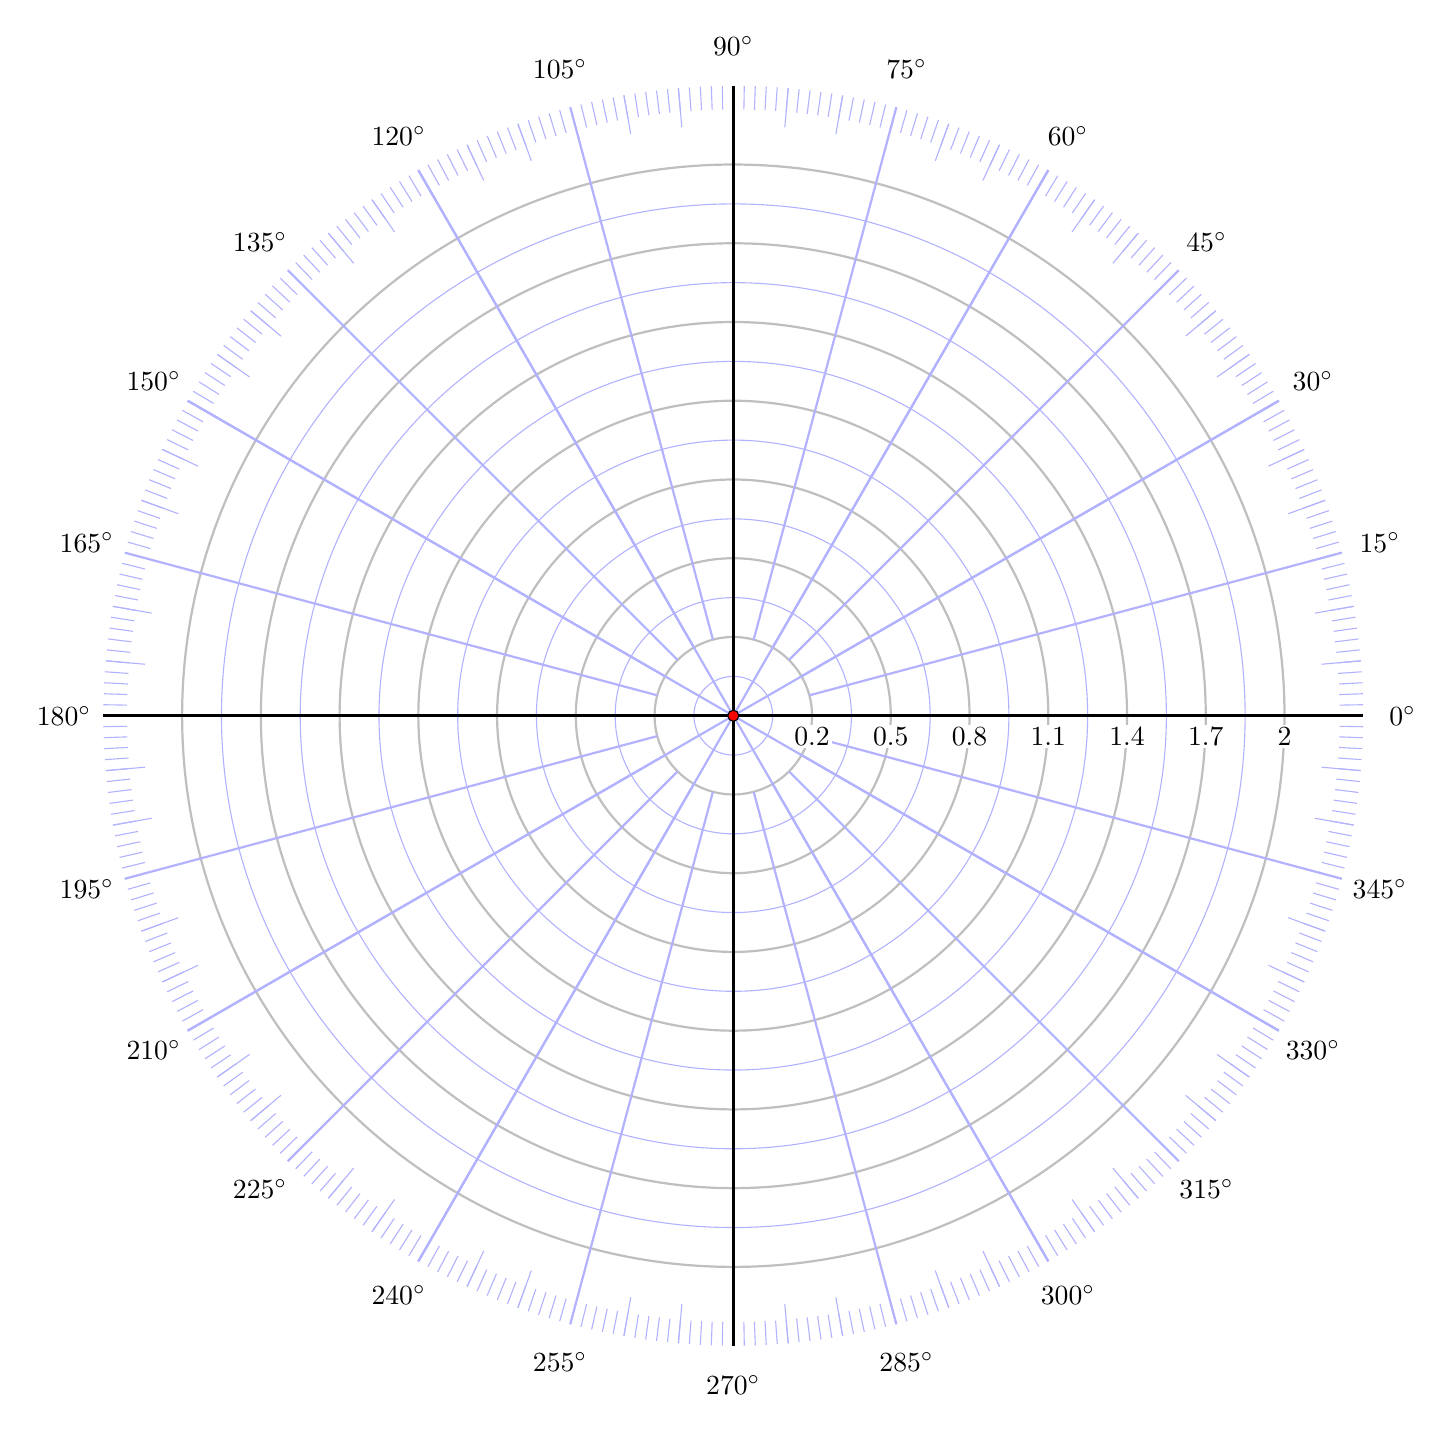
\begin{tikzpicture}
    %Circles 
    \foreach \r in {1, 2,...,7}
      \draw[gray!50, thick] (0,0) circle (\r);    
    \foreach \r in {0.5, 1.5,...,7}
      \draw[blue!30, thin] (0,0) circle (\r);
    %1¡ Rays
    \foreach \a in {0, 1,...,359}
      \draw[blue!30] (\a:7.7) -- (\a:8);
    %5¡ Rays
    \foreach \a in {0, 5,...,359}
      \draw[blue!30] (\a:7.5) -- (\a:8);      
    %15¡ Rays
    \foreach \a in {0, 15,...,359}
      \draw[thick,blue!30] (\a:1) -- (\a:8); 
    %30¡ Rays
    \foreach \a in {0, 30,...,359}
      \draw[thick,blue!30] (0, 0) -- (\a:8);
    %Radius labels (background filled white)
      \draw (1,0) node[inner sep=1pt,below=3pt,rectangle,fill=white] {$0.2$};
      \draw (2,0) node[inner sep=1pt,below=3pt,rectangle,fill=white] {$0.5$};
      \draw (3,0) node[inner sep=1pt,below=3pt,rectangle,fill=white] {$0.8$};
      \draw (4,0) node[inner sep=1pt,below=3pt,rectangle,fill=white] {$1.1$};
      \draw (5,0) node[inner sep=1pt,below=3pt,rectangle,fill=white] {$1.4$};
      \draw (6,0) node[inner sep=1pt,below=3pt,rectangle,fill=white] {$1.7$};
      \draw (7,0) node[inner sep=1pt,below=3pt,rectangle,fill=white] {$2$};
    %Main rays
    \foreach \a in {0, 90,...,359}
      \draw[very thick] (0, 0) -- (\a:8);
    %Angle labels  
    \foreach \a in {0, 15,...,359}
      \draw (\a: 8.5) node {$\a^\circ$};
    %Central point
    \draw[fill=red] (0,0) circle(0.7mm);
  \end{tikzpicture}
\end{center}
\pagebreak

\bonusprob{12} I like problems that involve lots of little graphs

\vskip1em
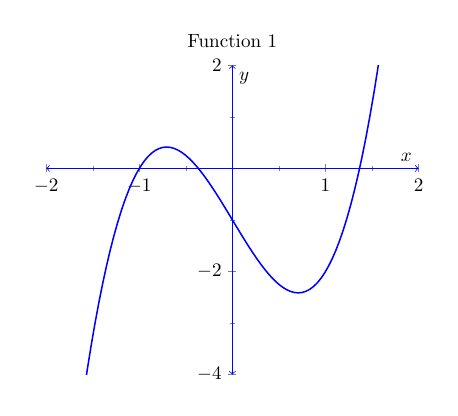
\begin{tikzpicture}[scale=0.69]
\begin{axis}[
	xmin=-2, xmax = 2,
	ymin=-4, ymax = 2,
	%xlabel={$x$},% ylabel={$y$},
	minor x tick num = {1},
	minor y tick num = {1},
	title={Function 1},
	scaled ticks=false,
	]
    \addplot[thick, color=blue, variable=\x, domain=-2:2, samples=100,unbounded coords=jump] 
        {2*x^3-3*x-1};
\end{axis}
\end{tikzpicture}
\hfill
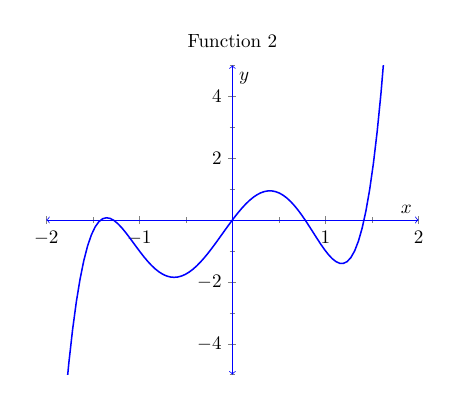
\begin{tikzpicture}[scale=0.69]
\begin{axis}[
	xmin=-2, xmax = 2,
	ymin=-5, ymax = 5,
	%xlabel={$x$},% ylabel={$y$},
	title={Function 2},
	minor x tick num = {1},
	minor y tick num = {1},
	scaled ticks=false,
	]
    \addplot[thick, color=blue, variable=\x, domain=-2:2, samples=100,unbounded coords=jump] 
        {2*x^5+1*x^4-6*x^3-2*x^2+4*x};
\end{axis}
\end{tikzpicture}
\hfill
\begin{tikzpicture}[scale=0.69]
\begin{axis}[
	xmin=-2, xmax = 2,
	ymin=-2, ymax = 2,
	%xlabel={$x$},% ylabel={$y$},
	minor x tick num = {1},
	minor y tick num = {1},
	title={Function 3},
	scaled ticks=false,
	]
    \addplot[thick, color=blue, variable=\x, domain=-2:2, samples=100,unbounded coords=jump] 
        {4*x^4+4*x^3+0.2*x^2+2*x};
\end{axis}
\end{tikzpicture}

%%
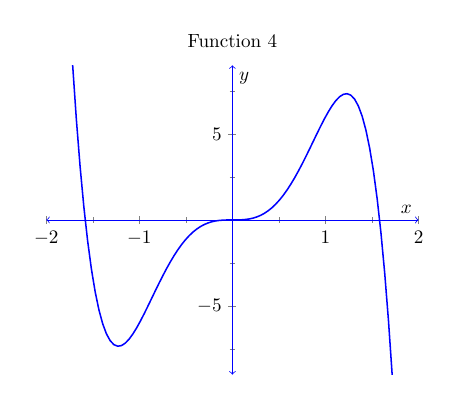
\begin{tikzpicture}[scale=0.69]
\begin{axis}[
	xmin=-2, xmax = 2,
	ymin=-9, ymax = 9,
	%xlabel={$x$},% ylabel={$y$},
	minor x tick num = {1},
	minor y tick num = {1},
	title={Function 4},
	scaled ticks=false,
	]
    \addplot[thick, color=blue, variable=\x, domain=-2:2, samples=100,unbounded coords=jump] 
        {-4*x^5+10*x^3};
\end{axis}
\end{tikzpicture}
\hfill
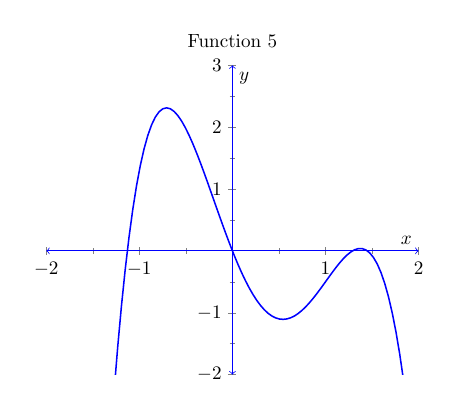
\begin{tikzpicture}[scale=0.69]
\begin{axis}[
	xmin=-2, xmax = 2,
	ymin=-2, ymax = 3,
	%xlabel={$x$},% ylabel={$y$},
	minor x tick num = {1},
	minor y tick num = {1},
	title={Function 5},
	scaled ticks=false,
	]
    \addplot[thick, color=blue, variable=\x, domain=-2:2, samples=100,unbounded coords=jump] 
        {-1.8*x^4+2.9*x^3+2.2*x^2-3.8*x};
\end{axis}
\end{tikzpicture}
\hfill
\begin{tikzpicture}[scale=0.69]
\begin{axis}[
	xmin=-2, xmax = 2,
	ymin=-8, ymax = 8,
	%xlabel={$x$},% ylabel={$y$},
	title={Function 6},
	minor x tick num = {1},
	minor y tick num = {1},
	scaled ticks=false,
	]
    \addplot[thick, color=blue, variable=\x, domain=-2:2, samples=100,unbounded coords=jump] 
        {-x^3};
\end{axis}
\end{tikzpicture}

%%%%%%%%%%%%%%%%%%%%%%%%%%%%%%%%%%%%%%%%%%%%%%%%%%%%%%%%%%%%%%%%%%%%%%%%%%%%%%%%%%%%%
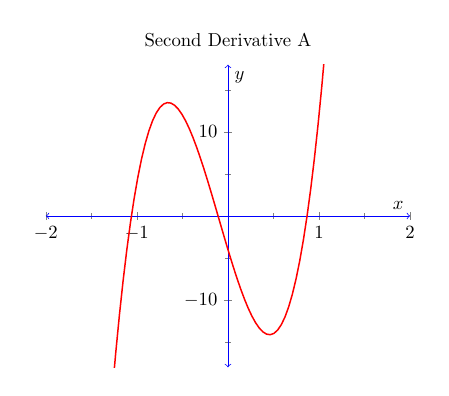
\begin{tikzpicture}[scale=0.675]
\begin{axis}[
	xmin=-2, xmax = 2,
	ymin=-18, ymax = 18,
	%xlabel={$x$},% ylabel={$y$},
	minor x tick num = {1},
	minor y tick num = {1},
	title={Second Derivative A},
	scaled ticks=false,
	]
    \addplot[thick, color=red, variable=\x, domain=-2:2, samples=100,unbounded coords=jump] 
        {40*x^3+12*x^2-36*x-4};
\end{axis}
\end{tikzpicture}
\hfill
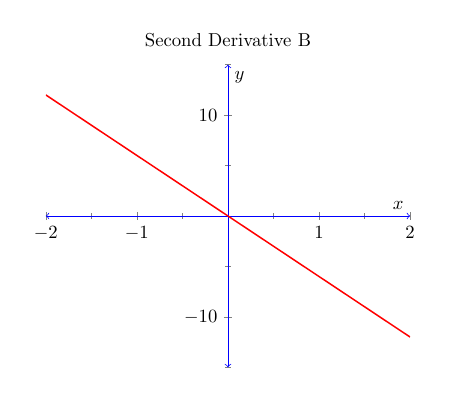
\begin{tikzpicture}[scale=0.675]
\begin{axis}[
	xmin=-2, xmax = 2,
	ymin=-15, ymax = 15,
	%xlabel={$x$},% ylabel={$y$},
	title={Second Derivative B},
	minor x tick num = {1},
	minor y tick num = {1},
	scaled ticks=false,
	]
    \addplot[thick, color=red, variable=\x, domain=-2:2, samples=100,unbounded coords=jump] 
        {-6*x};
\end{axis}
\end{tikzpicture}
\hfill
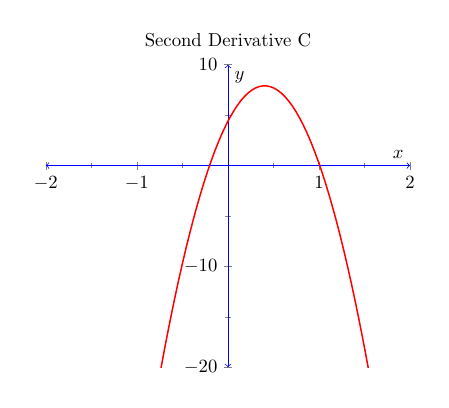
\begin{tikzpicture}[scale=0.675]
\begin{axis}[
	xmin=-2, xmax = 2,
	ymin=-20, ymax = 10,
	%xlabel={$x$},% ylabel={$y$},
	minor x tick num = {1},
	minor y tick num = {1},
	title={Second Derivative C},
	scaled ticks=false,
	]
    \addplot[thick, color=red, variable=\x, domain=-2:2, samples=100,unbounded coords=jump] 
        {-21.6*x^2+17.4*x+4.4};
\end{axis}
\end{tikzpicture}

%%
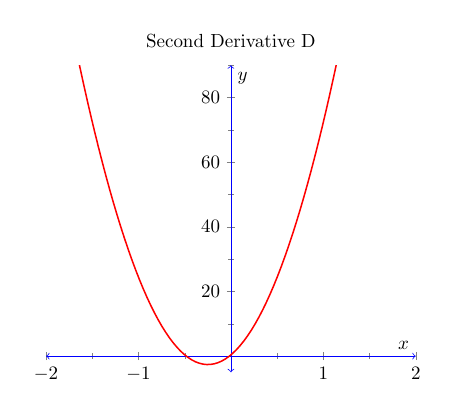
\begin{tikzpicture}[scale=0.685]
\begin{axis}[
	xmin=-2, xmax = 2,
	ymin=-5, ymax = 90,
	%xlabel={$x$},% ylabel={$y$},
	minor x tick num = {1},
	minor y tick num = {1},
	title={Second Derivative D},
	scaled ticks=false,
	]
    \addplot[thick, color=red, variable=\x, domain=-2:2, samples=100,unbounded coords=discard] 
        {48*x^2+24*x+0.4};
\end{axis}
\end{tikzpicture}
\hfill
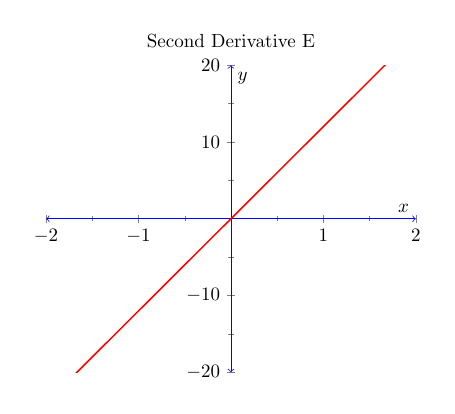
\begin{tikzpicture}[scale=0.685]
\begin{axis}[
	xmin=-2, xmax = 2,
	ymin=-20, ymax = 20,
	%xlabel={$x$},% ylabel={$y$},
	title={Second Derivative E},
	minor x tick num = {1},
	minor y tick num = {1},
	scaled ticks=false,
	]
    \addplot[thick, color=red, variable=\x, domain=-2:2, samples=101,unbounded coords=jump] 
        {12*x};
\end{axis}
\end{tikzpicture}
\hfill
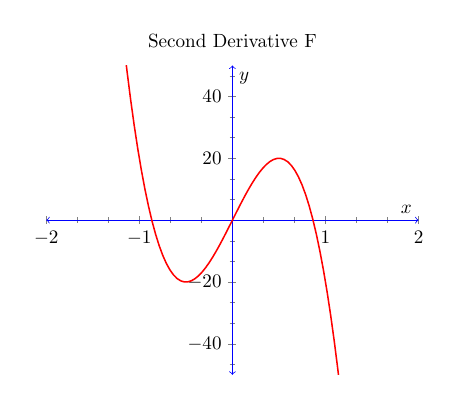
\begin{tikzpicture}[scale=0.69]
\begin{axis}[
	xmin=-2, xmax = 2,
	ymin=-50, ymax = 50,
	%xlabel={$x$},% ylabel={$y$},
	minor x tick num = {2},
	minor y tick num = {2},
	title={Second Derivative F},
	scaled ticks=false,
	]
    \addplot[thick, color=red, variable=\x, domain=-1.9:1.9, samples=100,unbounded coords=jump] 
        {20*x*(-4*x^2+3)};
\end{axis}
\end{tikzpicture}

\vskip1em
Function 1 matches Second Derivative \rule{2em}{0.5pt}
$\qquad$
Function 4 matches Second Derivative \rule{2em}{0.5pt}

Function 2 matches Second Derivative \rule{2em}{0.5pt}
$\qquad$
Function 5 matches Second Derivative \rule{2em}{0.5pt}

Function 3 matches Second Derivative \rule{2em}{0.5pt}
$\qquad$
Function 6 matches Second Derivative \rule{2em}{0.5pt}

\pagebreak

\end{enumerate}
% End writing points table in separate tex file----------------
\immediate\write\pointstable{TOTAL (\arabic{PointCount} pts)\unexpanded{&\quad\quad\quad\quad\quad\quad\\ &\\ \hline}}
\immediate\write\pointstable{\unexpanded{\end{tabular} \end{center}}}
\immediate\closeout\pointstable
%--------------------------------------------------------------
\end{document}